\documentclass[11pt]{beamer}
%Gummi|065|=)
\usepackage[T1]{fontenc}
\usepackage{graphicx}
\usepackage[absolute]{textpos}
\usepackage{amsfonts,amssymb,amsmath,amsthm}
\usepackage{amsbsy}
\usepackage[UKenglish]{babel}
\usepackage[round,authoryear,sort]{natbib}
\usepackage[T1]{fontenc} % Handles accents etc better in the invisible details of the pdf output.
\usepackage[UKenglish]{babel} % Let LaTeX know what language the text is in so it can select the correct hyphenation pattern etc
\usepackage{lmodern} % Load the latin modern set of fonts


\usetheme{Madrid}
\usecolortheme{default}
\useinnertheme{circles}

\definecolor{Logo1}{rgb}{0.208, 0.2865, 0.373}
\definecolor{Logo2}{rgb}{0.000, 0.674, 0.863}

\setbeamercolor*{palette primary}{bg=Logo1, fg=white}
\setbeamercolor*{palette secondary}{bg=Logo2, fg=white}
\setbeamercolor*{palette tertiary}{bg=white, fg=Logo1}
\setbeamercolor*{palette quaternary}{bg=Logo1,fg=white}
\setbeamercolor{structure}{fg=Logo1} % itemize, enumerate, etc
\setbeamercolor{section in toc}{fg=Logo1} % TOC sections

\makeatletter
\newcommand*{\supervisor}[1]{\gdef\@supervisor{#1}}
\newcommand*{\logoimg}[1]{\gdef\@logoimg{#1}}


\graphicspath{ {/home/thomasc/uni/thesis/viva} }

\title[Data Aggregation]{The Effect of Data Aggregation on Statistical Inference}
\author[Thomas Crow]{\Large {Thomas Crow \\ \footnotesize Supervisor: Ed Cohen}}
\date{\today}
\titlegraphic{
\includegraphics[height=.5cm]{Imperial_4_colour_process.jpg}}

\begin{document}

\maketitle

\begin{frame}
\frametitle{Table of Contents}
\tableofcontents
\end{frame}

\section{Motivation}
\begin{frame}
	\frametitle{Motivation - Microscopy}

	\begin{columns}

	\column{0.5\textwidth}
		\begin{itemize}
			\item Estimating position of fluorescing molecule with microscopy.
			\item Images are captured using counts within pixels, not with infinite precision.
			\item Non-explicit likelihood functions derived in \cite{localization_accuracy}.
		\end{itemize}
	\column{0.5\textwidth}
		\begin{figure}[!h]
			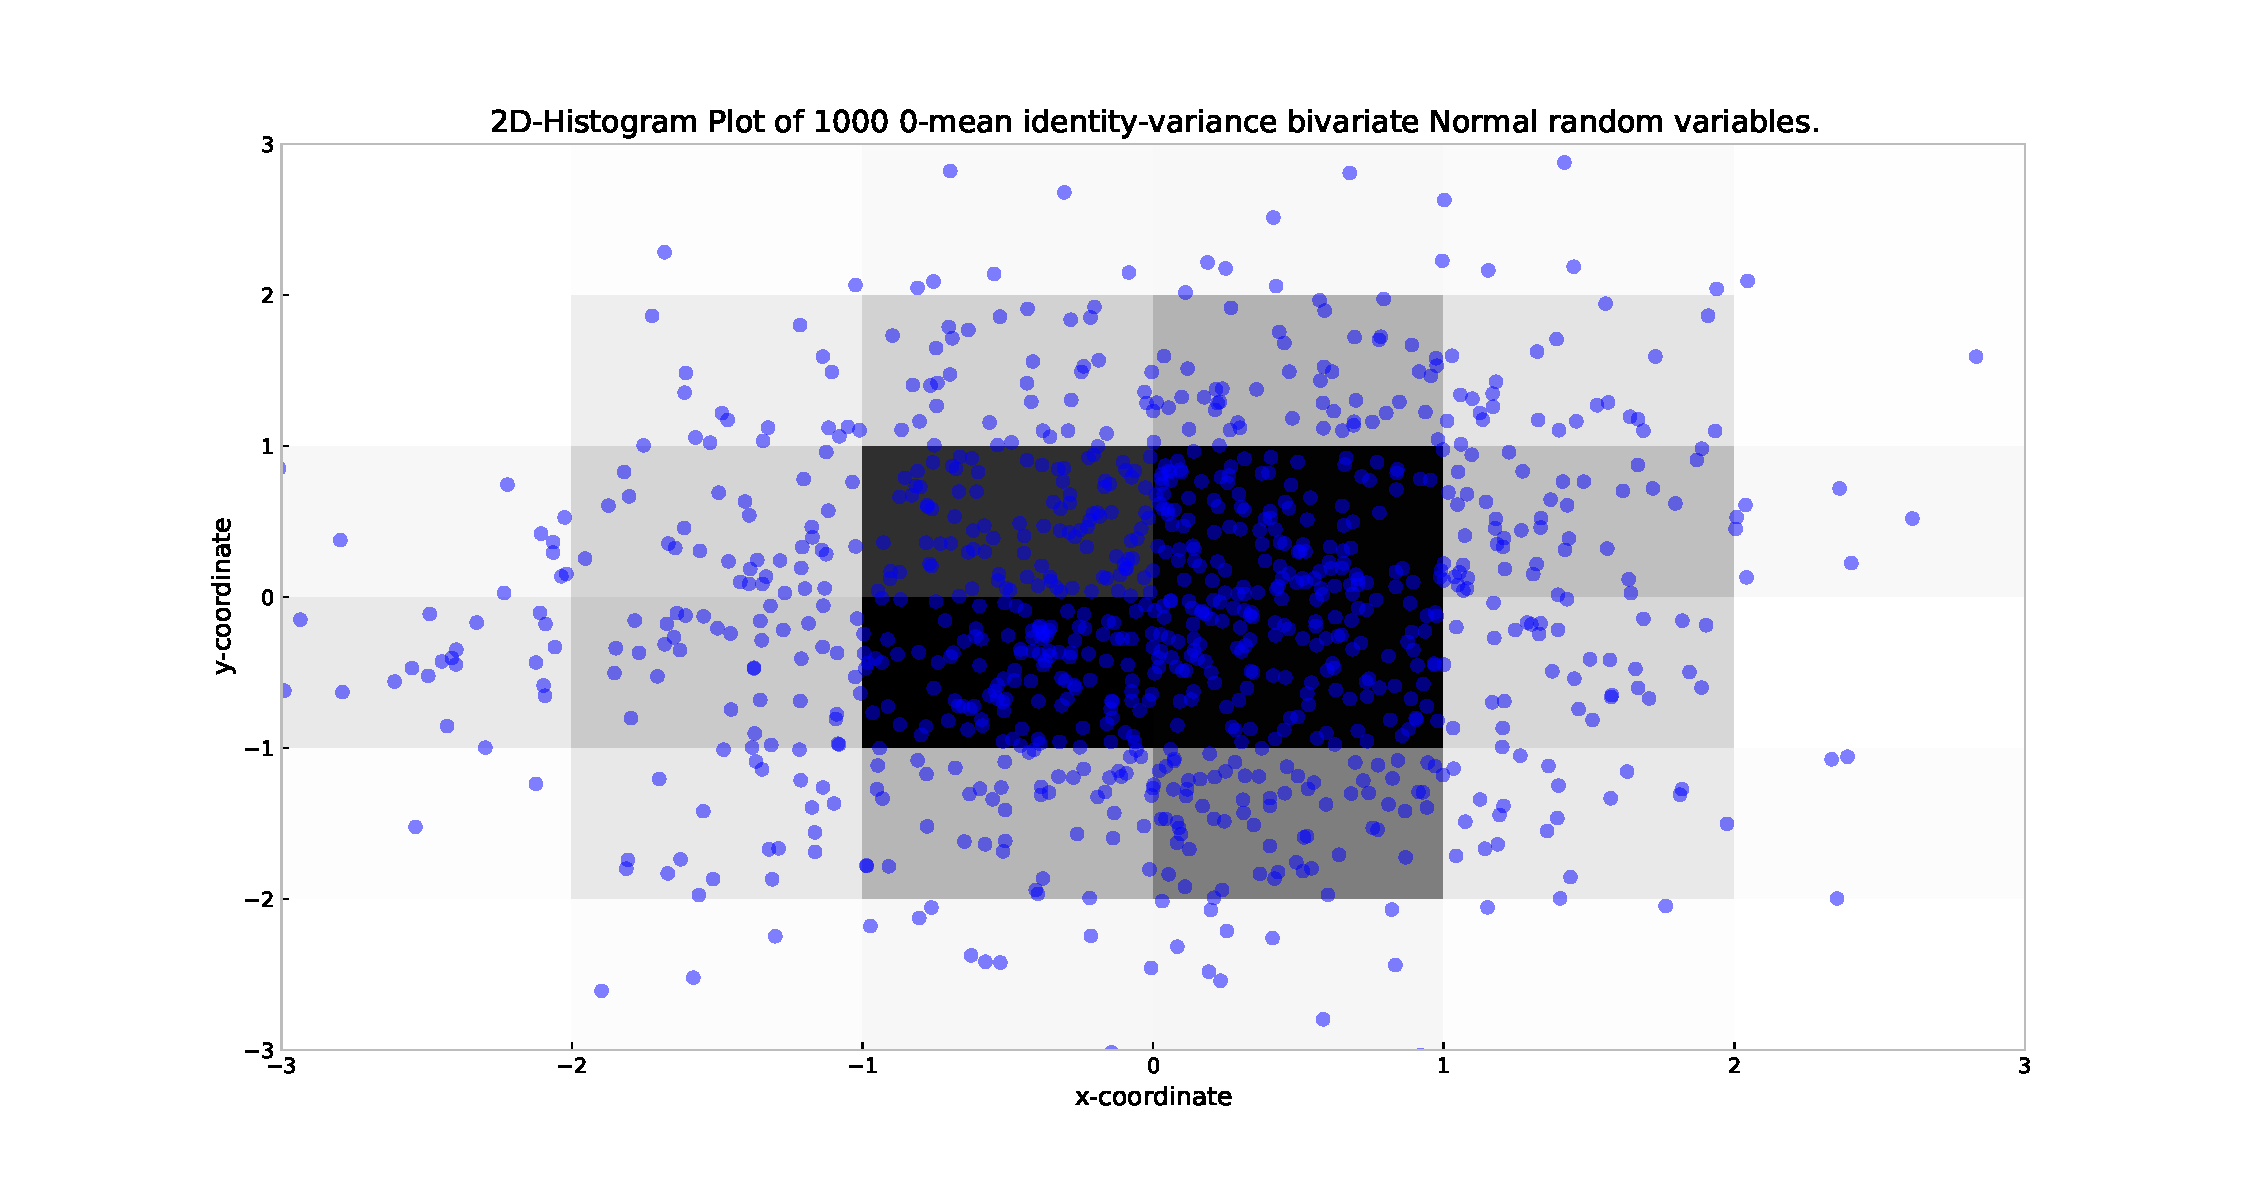
\includegraphics[height=6.5cm, width=6.5cm]{2d_pixel.pdf}
			\centering
		\end{figure}
		
	\end{columns}
\end{frame}

\begin{frame}
	\frametitle{Motivation - Stochastic Processes}
		\begin{itemize}
			\item Estimating parameters for rate function in Poisson process. E.g. estimating the number of incoming calls over the day to a telephone service.
			\item Can't store timestamps to infinite precision, may just have number of calls per minute, or hour.
		\end{itemize}
		\centering
		\begin{figure}[!h]
			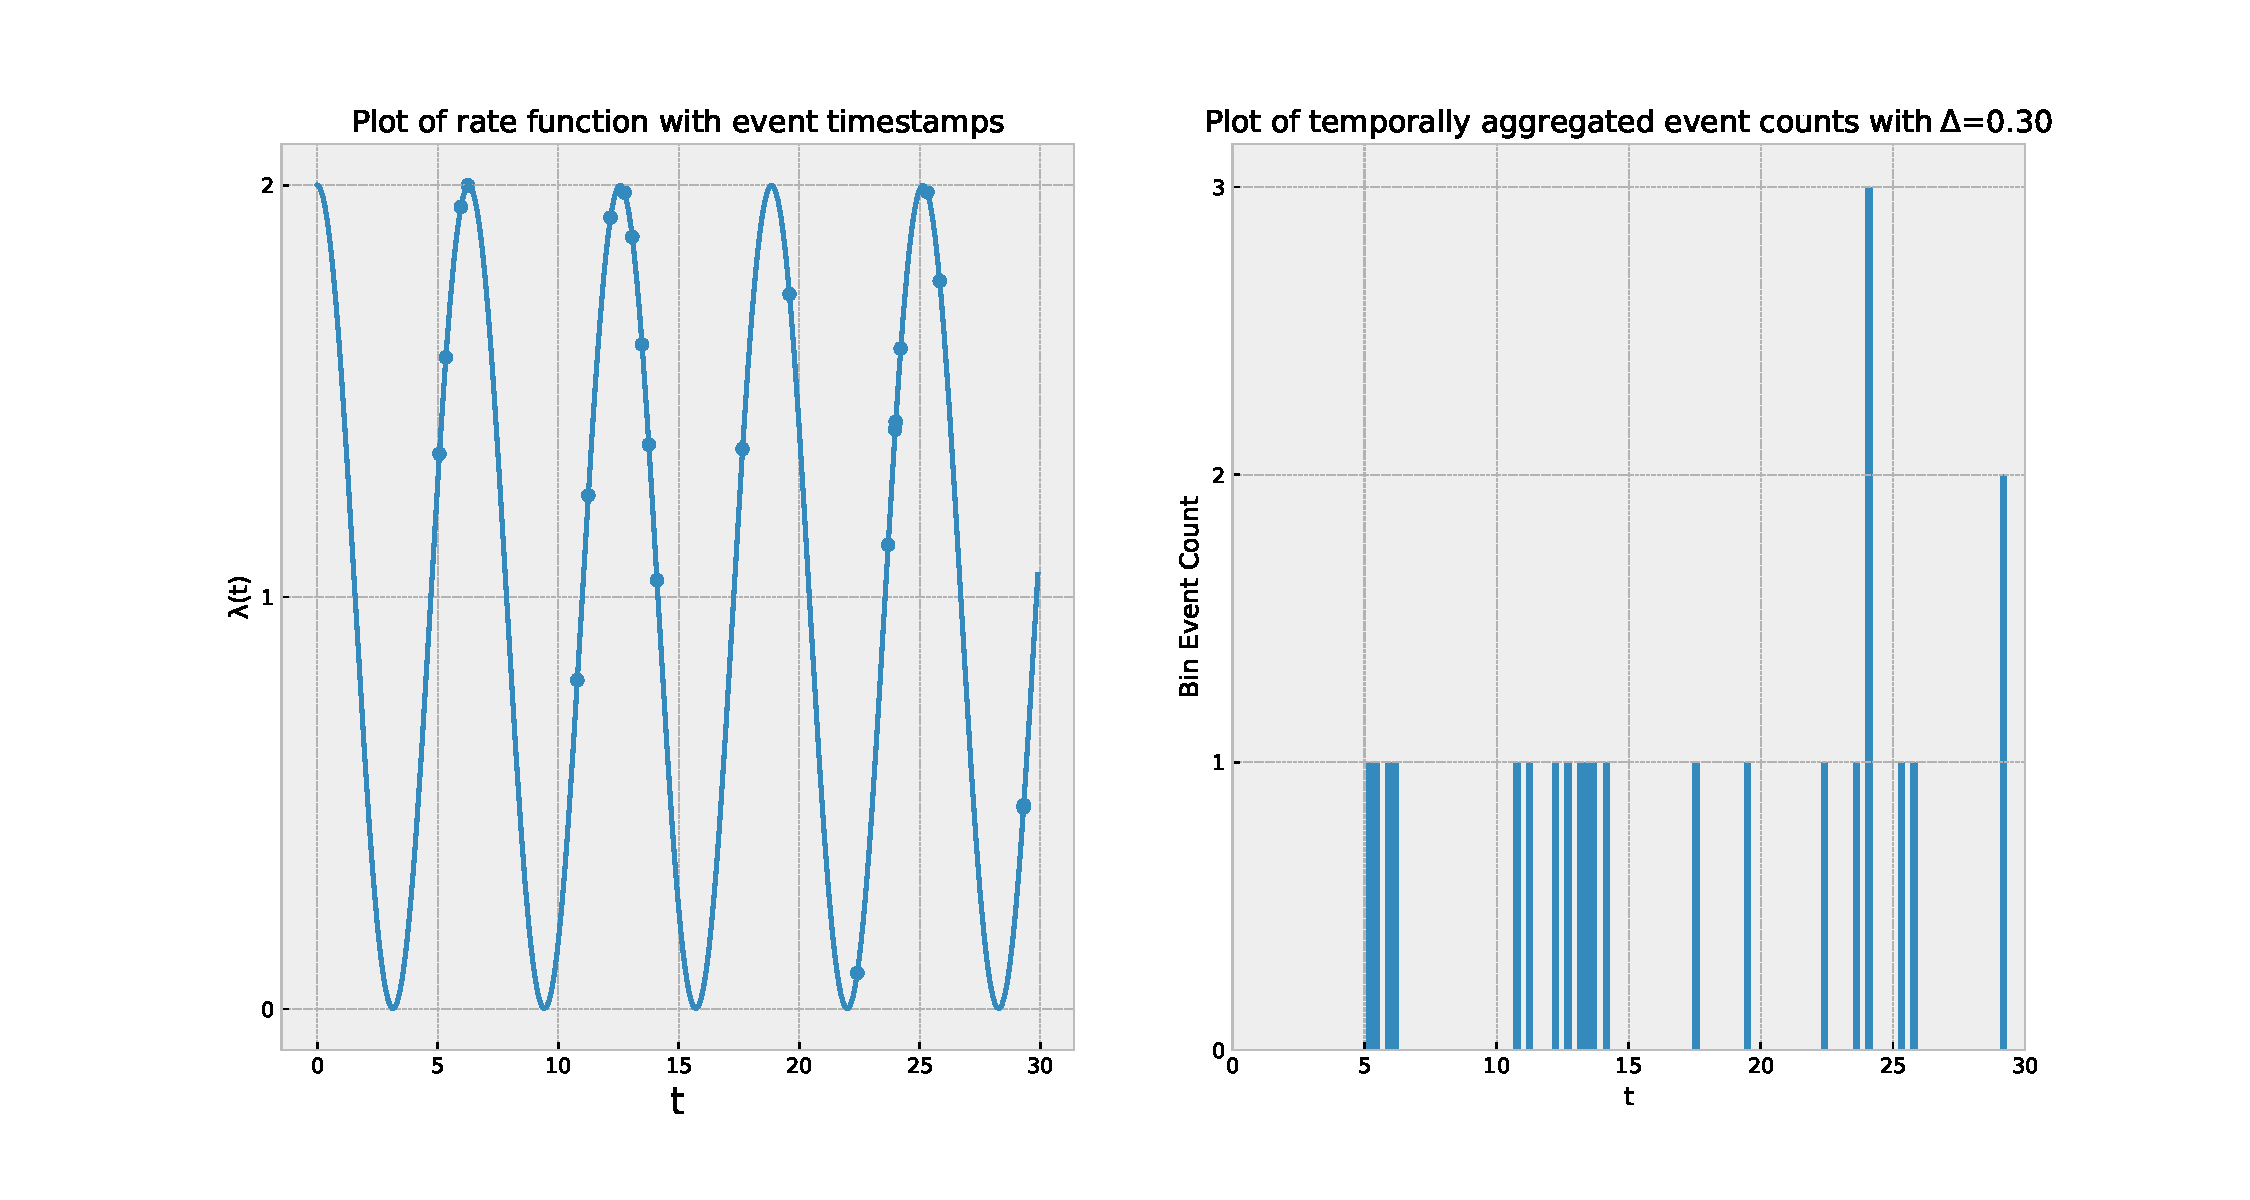
\includegraphics[height=4cm, width=12cm]{nhpp_periodic.pdf}
			\centering
		\end{figure}
\end{frame}

\begin{frame}
	\frametitle{General Approach}
	\begin{itemize}
		\item Random variable $X$ following some parametric distribution with density function $f(x; \theta)$ and distribution function $F(x; \theta)$.
		\item To calculate probability of an observation falling in $\Delta$-sized bin $B_k$ (with edges $(k \Delta, (k+1) \Delta]$):
		\begin{equation*}
			\mathbb{P}(x \in B_k; \theta) = \int_{x=k \Delta}^{(k+1)\Delta} f(x) \text{d} x = F((k+1) \Delta) - F(k \Delta).
		\end{equation*}
		\item Use this probability with observed counts $n_k$ in each bin to calculate binned log-likelihood:
		\begin{equation*}
			\ell(\theta; n_{-\infty}, \dots, n_{\infty}) = \sum_{k=-\infty}^\infty n_k \log \left( \mathbb{P}(x \in B_k; \theta) \right).
		\end{equation*}
	\end{itemize}
\end{frame}


\section{Likelihood Theory \& Identifiability}

\begin{frame}
	\frametitle{Likelihood Theory}
	\begin{itemize}
		\item Estimating parameter $\theta$ given i.i.d data $x_1,\dots,x_n$. Maximise log-likelihood $\ell(\theta; x_1,\dots,x_n)$.
		\item MLE $\hat{\theta}$ at $\nabla_{\theta}\ell(\theta)=0$.
		\item Hessian $\mathbf{H} = \nabla_{\theta}\nabla_{\theta}^T \ell(\theta)$.
		\item Fisher Information $\mathcal{I}(\theta) = - \mathbb{E}\left[\mathbf{H}\right]$.
		\item Cram\'er-Rao Lower Bound [\cite{rao_crlb}]:
		\begin{equation*}
			\text{Var}(\hat{\theta}) \geq \mathcal{I}^{-1}(\theta),
		\end{equation*}
		gives lower limit for asymptotic variance of MLE.
	\end{itemize}
\end{frame}


\begin{frame}
	\frametitle{Identifiability}
	\begin{itemize}
		\item Global identifiability is when there exists a unique mapping from parameter space to model space.
		\item Unidentifiability often occurs due to different parameters achieving the maximum likelihood.
		\item Fisher Information matrix is non-singular if and only if $\theta$ is locally identifiable, that is:
		\begin{equation*}
			\ell(\theta; x_1, \dots, x_n) = \ell(\phi; x_1, \dots, x_n) \implies \theta = \phi,
		\end{equation*}
		in a neighbourhood around $\theta$ [\cite{rothenburg_1971}].
	\end{itemize}
\end{frame}

\section{Exponential Distribution}

\begin{frame}
	\frametitle{Exponential Distribution}
	\begin{itemize}
		\item Random variable $X$ follows Exponential($\lambda$) distribution if:
		\begin{equation*}
			f(x; \lambda) = \lambda e^{- \lambda x}, \quad \quad x \geq 0, \lambda > 0.
		\end{equation*}
		\item Fisher Information for $\lambda$ is given in both cases as:
		\begin{equation*}
			\mathcal{I}_{cts}(\lambda) = \frac{n}{\lambda^2}, \quad \mathcal{I}_{bin}(\lambda) = \frac{n \Delta^2}{(e^{\Delta \lambda} - 1)^2}.
	\end{equation*}
	\end{itemize}
\end{frame}

\begin{frame}
	\frametitle{Exponential Fisher Information}
	\begin{itemize}
		\item As $\Delta$ increases, proportion of lost Fisher Information quickly approaches 1.
		\item Smaller values of $\lambda$ have greater variance, so aggregation has less relative effect.
	\end{itemize}
	\begin{figure}[!h]
		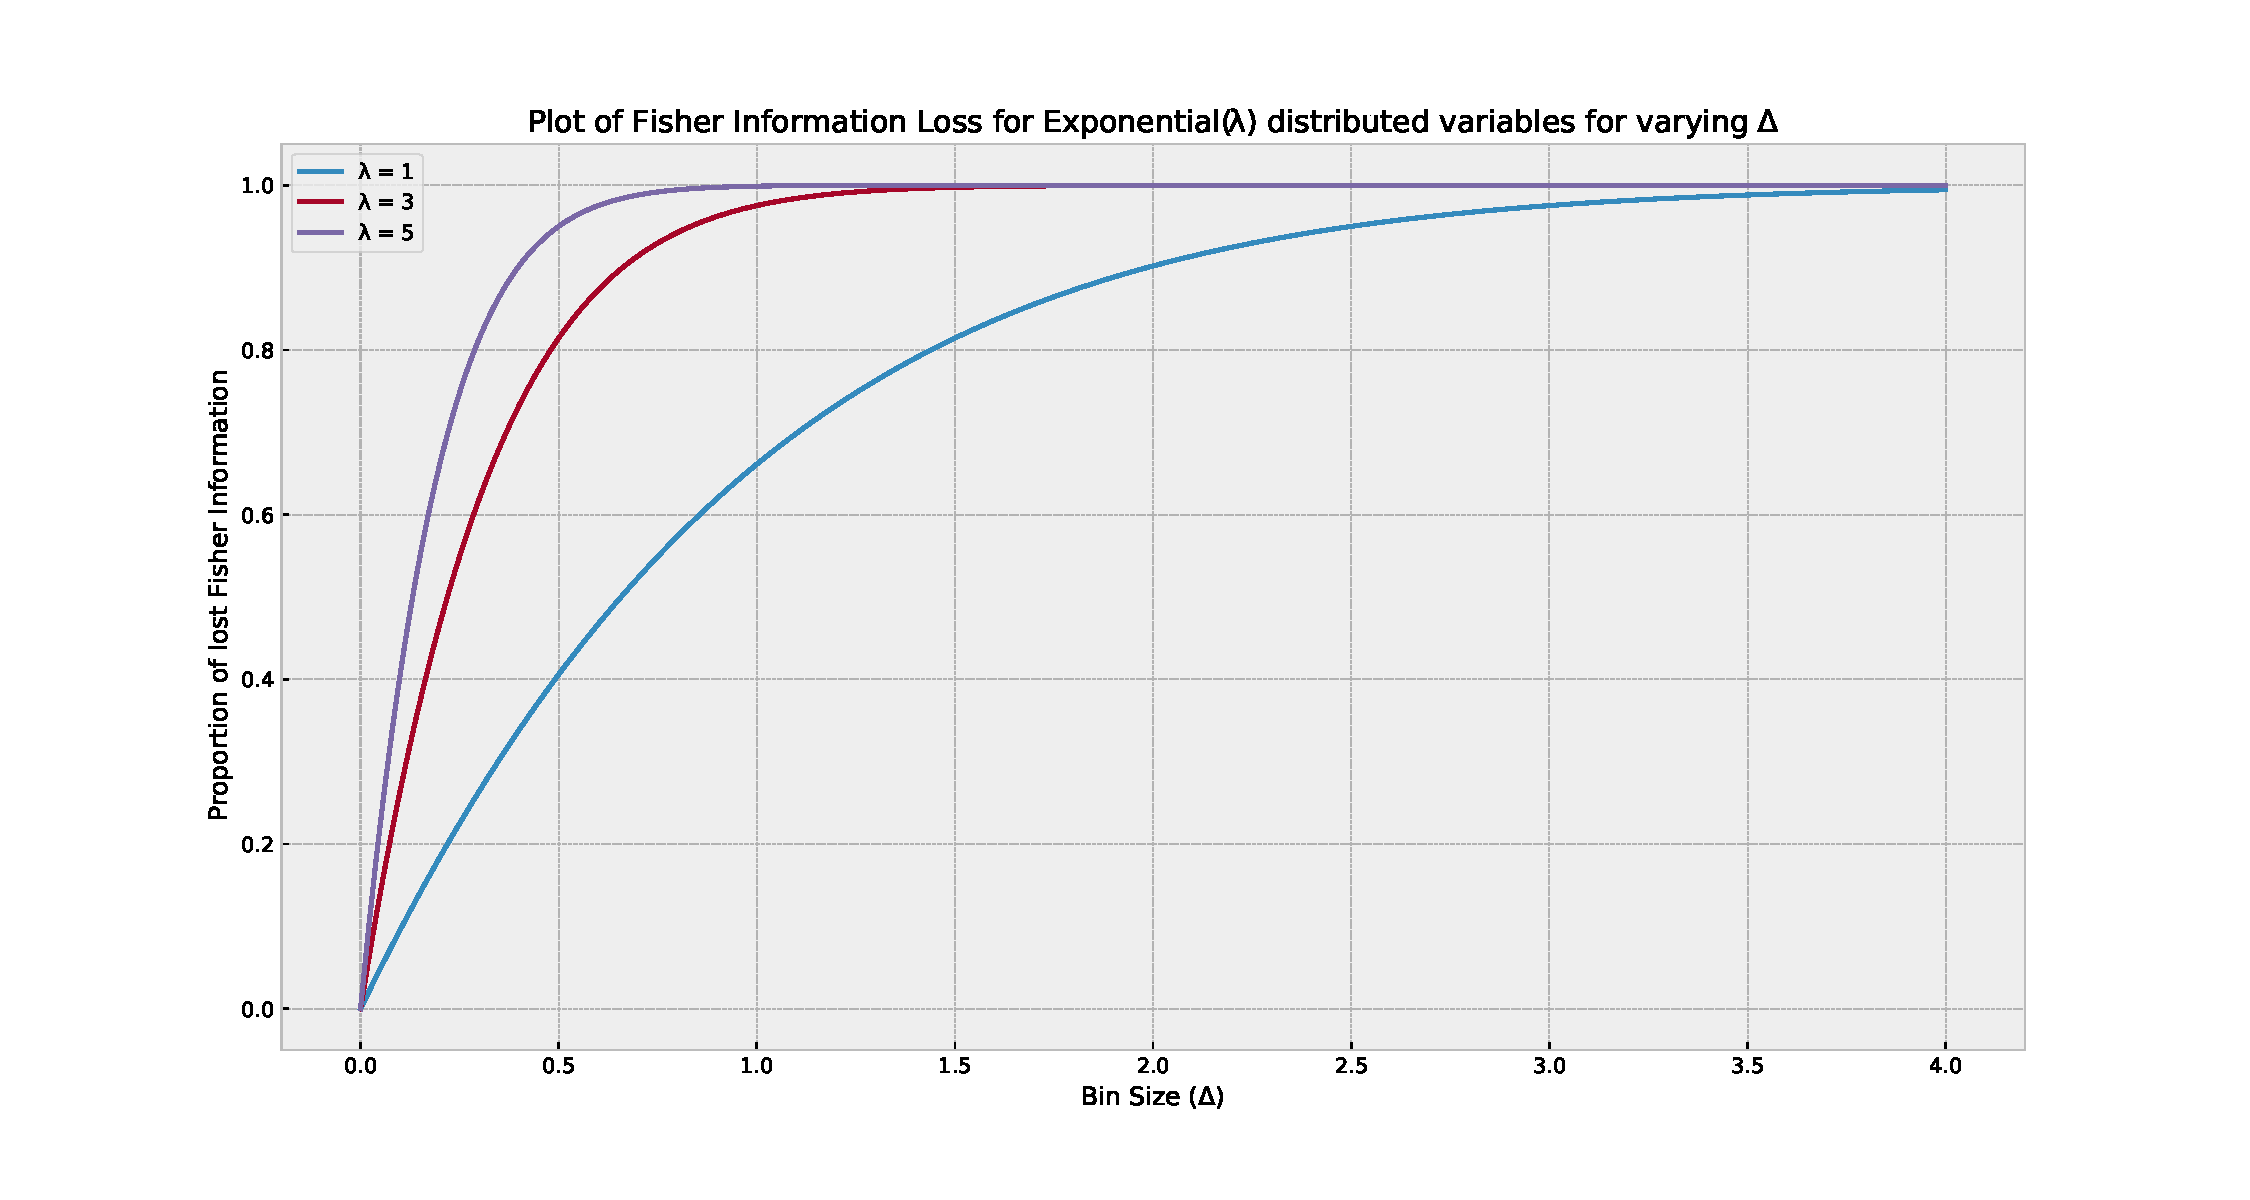
\includegraphics[height=5.5cm, width=12cm]{exp_info_loss.pdf}
	\end{figure}
\end{frame}

\begin{frame}
	\frametitle{Exponential Log-Likelihood Example}
	\begin{itemize}
		\item Loss of Fisher Information means flattening of log-likelihood curve around the MLE.
		\item Results in a higher variance MLE due to the CRLB.
	\end{itemize}
	\begin{figure}[!h]
		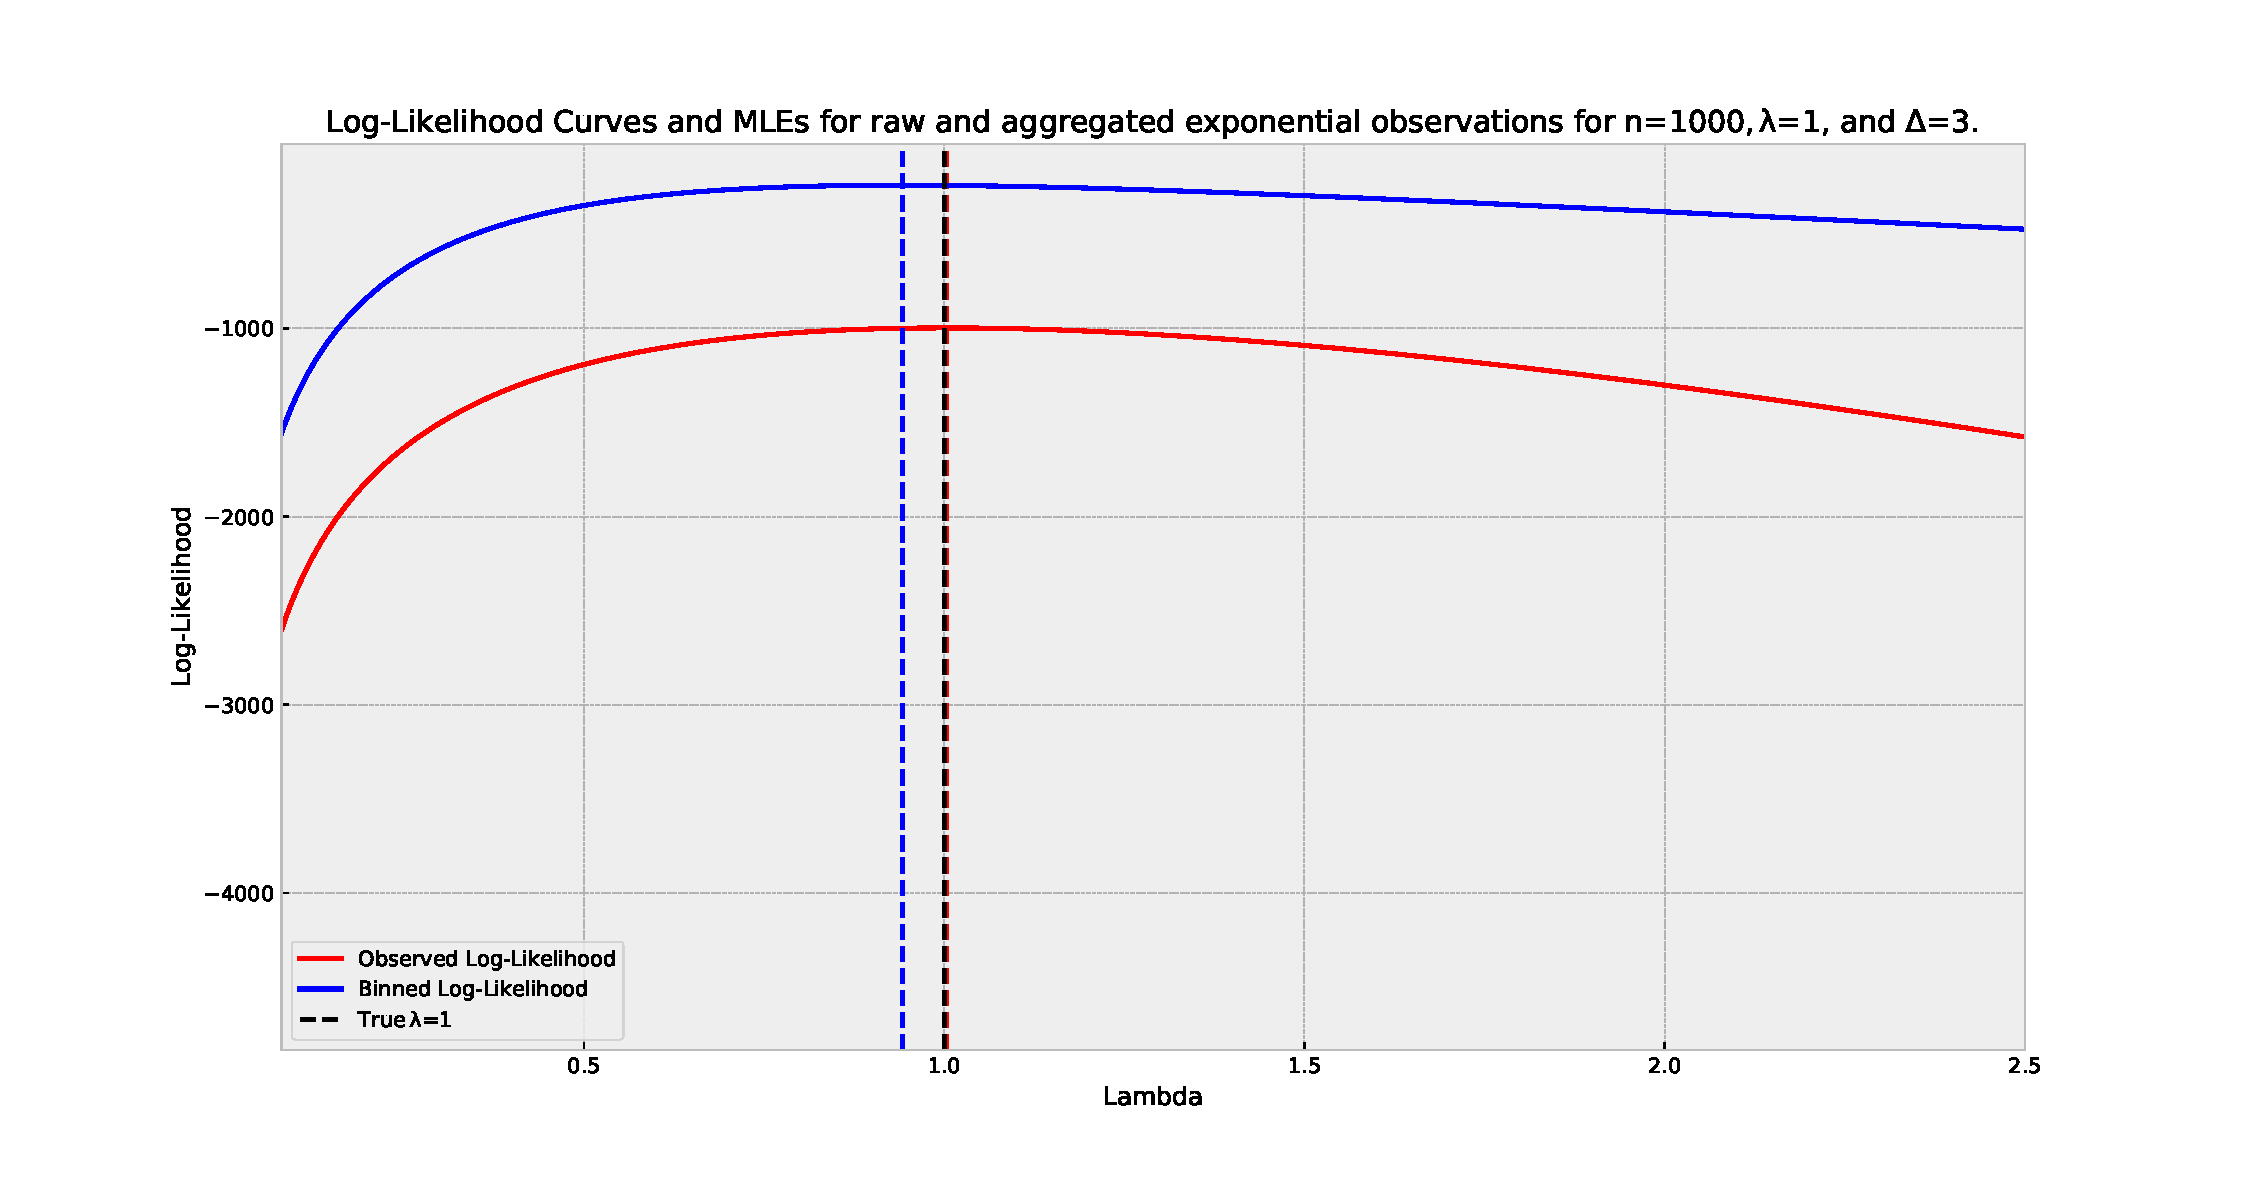
\includegraphics[height=6cm, width=12cm]{exp_log_likelihood.pdf}
	\end{figure}
\end{frame}


\section{Normal Distribution}

\begingroup
\small
\begin{frame}
	\frametitle{Normal Fisher Information - Aggregated Values}
	\begin{itemize}
	\item Random variable $X$ follows a $\mathcal{N}(\mu, \sigma)$ distribution if:
	\begin{equation*}
		f(x; \mu, \sigma^2) = \frac{1}{\sqrt{2 \pi \sigma^2}} \exp\left(-\frac{(x - \mu)^2}{2 \sigma^2} \right), \quad \quad x, \mu \in \mathbb{R}, \sigma > 0.
	\end{equation*}
	\item Fisher Information for $\mu$ given by:
	\begin{equation*}
			\mathcal{I}_{cts}(\mu) = \frac{n}{\sigma^2},
	\end{equation*}
	and
	\begin{equation*}
		\begin{aligned}
			&\mathcal{I}_{bin}(\mu) = \frac{n}{\sigma^2} \sum_{k=-\infty}^\infty 
			 \frac{\left(\phi \left( \frac{(k + 1) \Delta - \mu}{\sigma} \right) - \phi \left( \frac{k \Delta - \mu}{\sigma} \right)\right)^2}
			 {\Phi \left( \frac{(k + 1) \Delta - \mu}{\sigma} \right) - \Phi \left(\frac{k \Delta - \mu}{\sigma} \right)}
			  \\
			&- \frac{n}{\sigma^3} \sum_{k=-\infty}^\infty \left(
				((k + 1) \Delta - \mu) \phi \left( \frac{(k + 1) \Delta - \mu}{\sigma} \right) - (k \Delta - \mu) \phi \left( \frac{k \Delta - \mu}{\sigma} \right)
			\right).
		\end{aligned}
	\end{equation*}.
	\item Derivation also calculated for $\sigma$ Fisher Information. Off-diagonals are 0.
	\end{itemize}
\end{frame}
\endgroup

\begin{frame}
	\frametitle{Normal Fisher Information - Loss}
	\begin{itemize}
		\item Again, information loss increases as aggregation increases.
		\item Inference performance depends on both bin size ($\Delta$) and alignment of the bin edges with $\mu$.
	\end{itemize}
	\begin{columns}
	\column{0.5\textwidth}
		\begin{figure}[!h]
			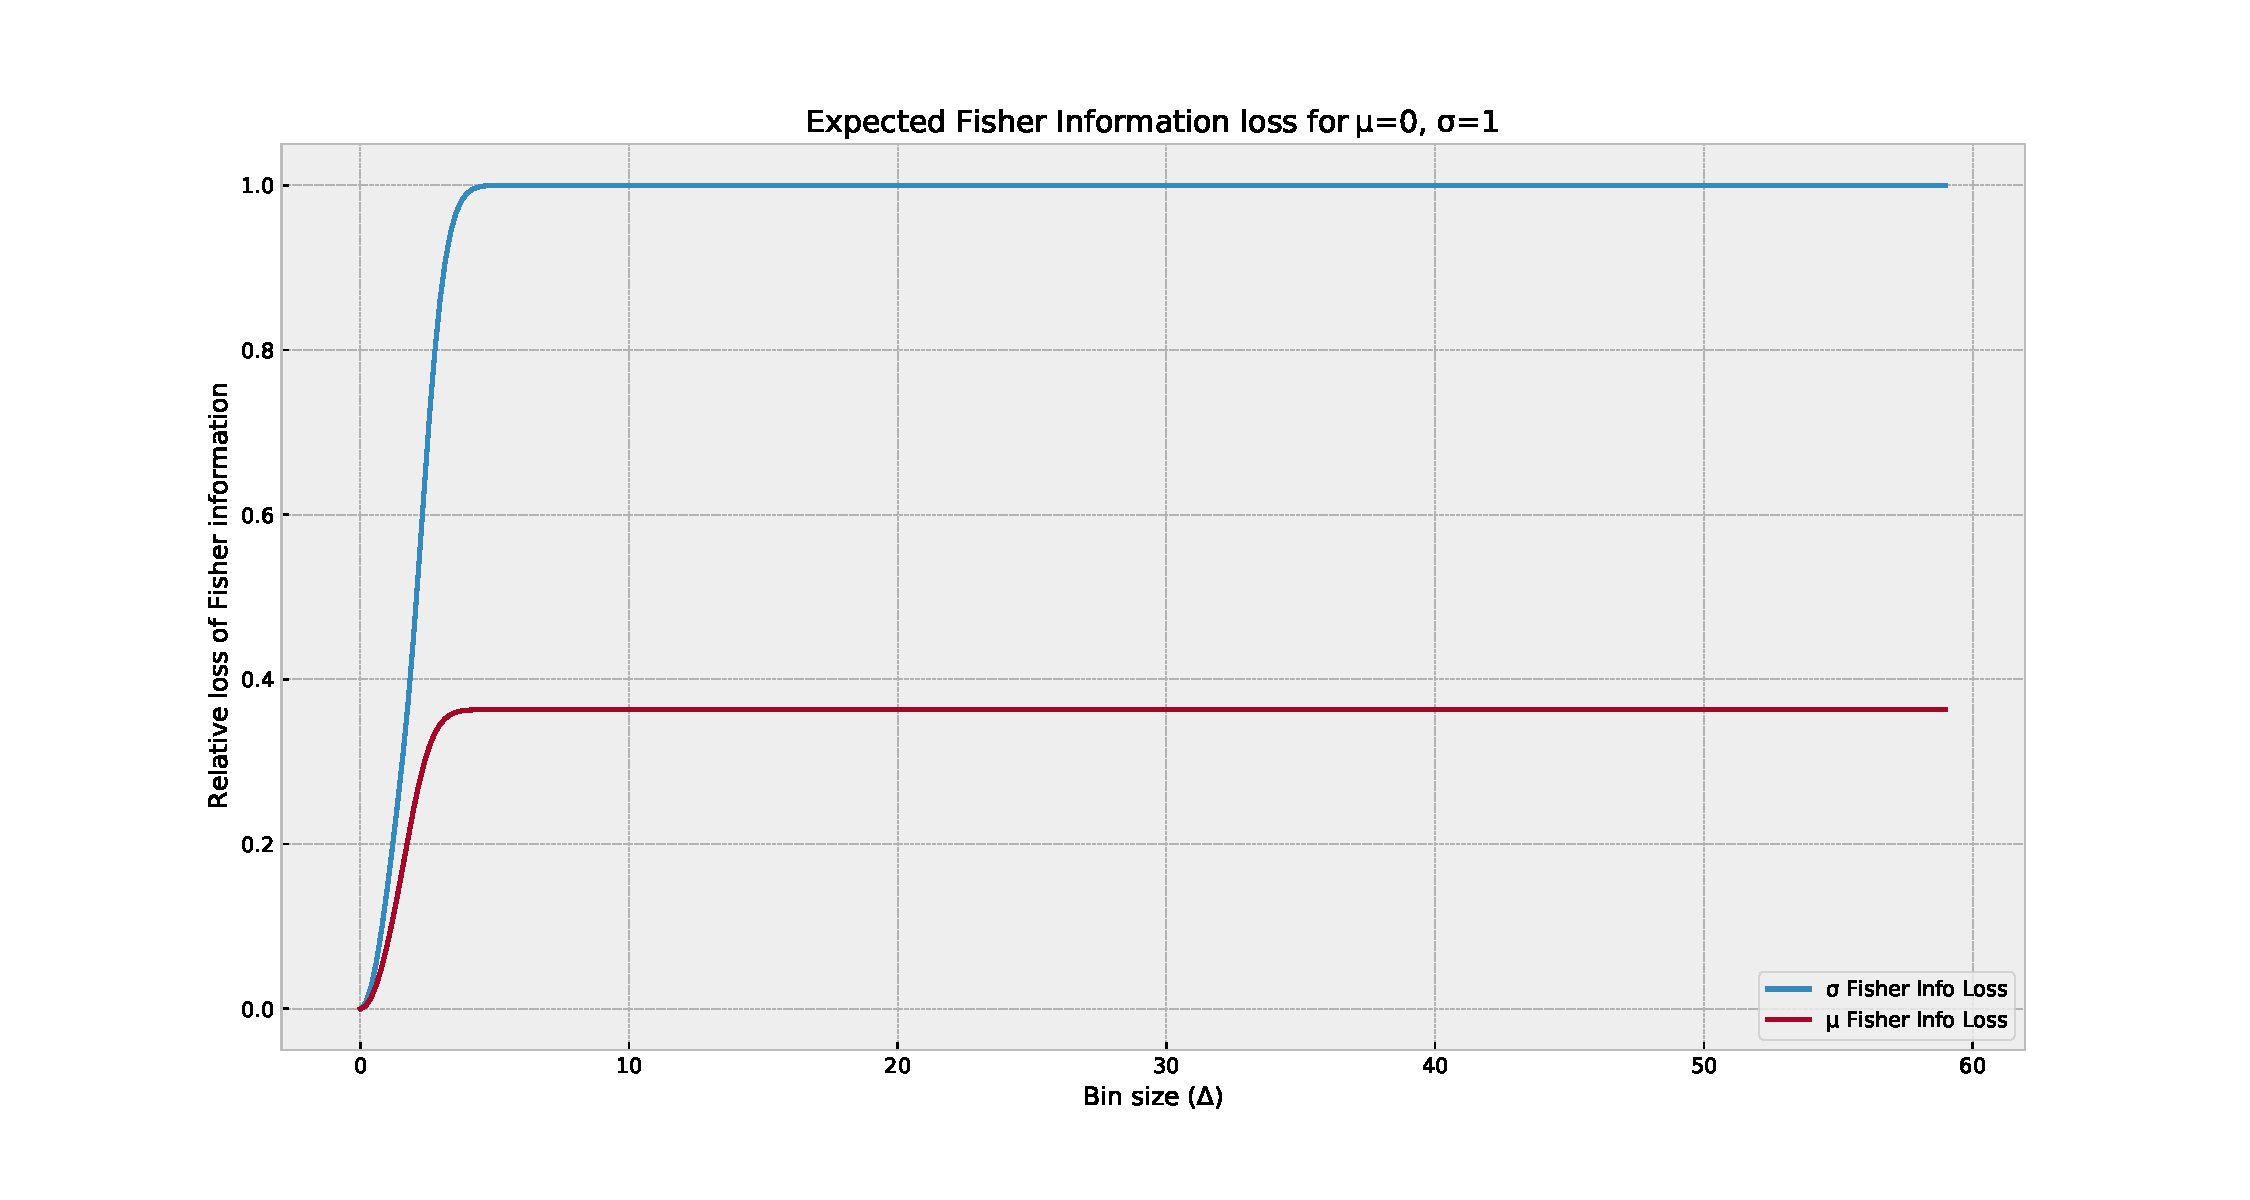
\includegraphics[height=5cm, width=6cm]{mu0sig1.pdf}
			\centering
		\end{figure}
	\column{0.5\textwidth}
		\begin{figure}[!h]
			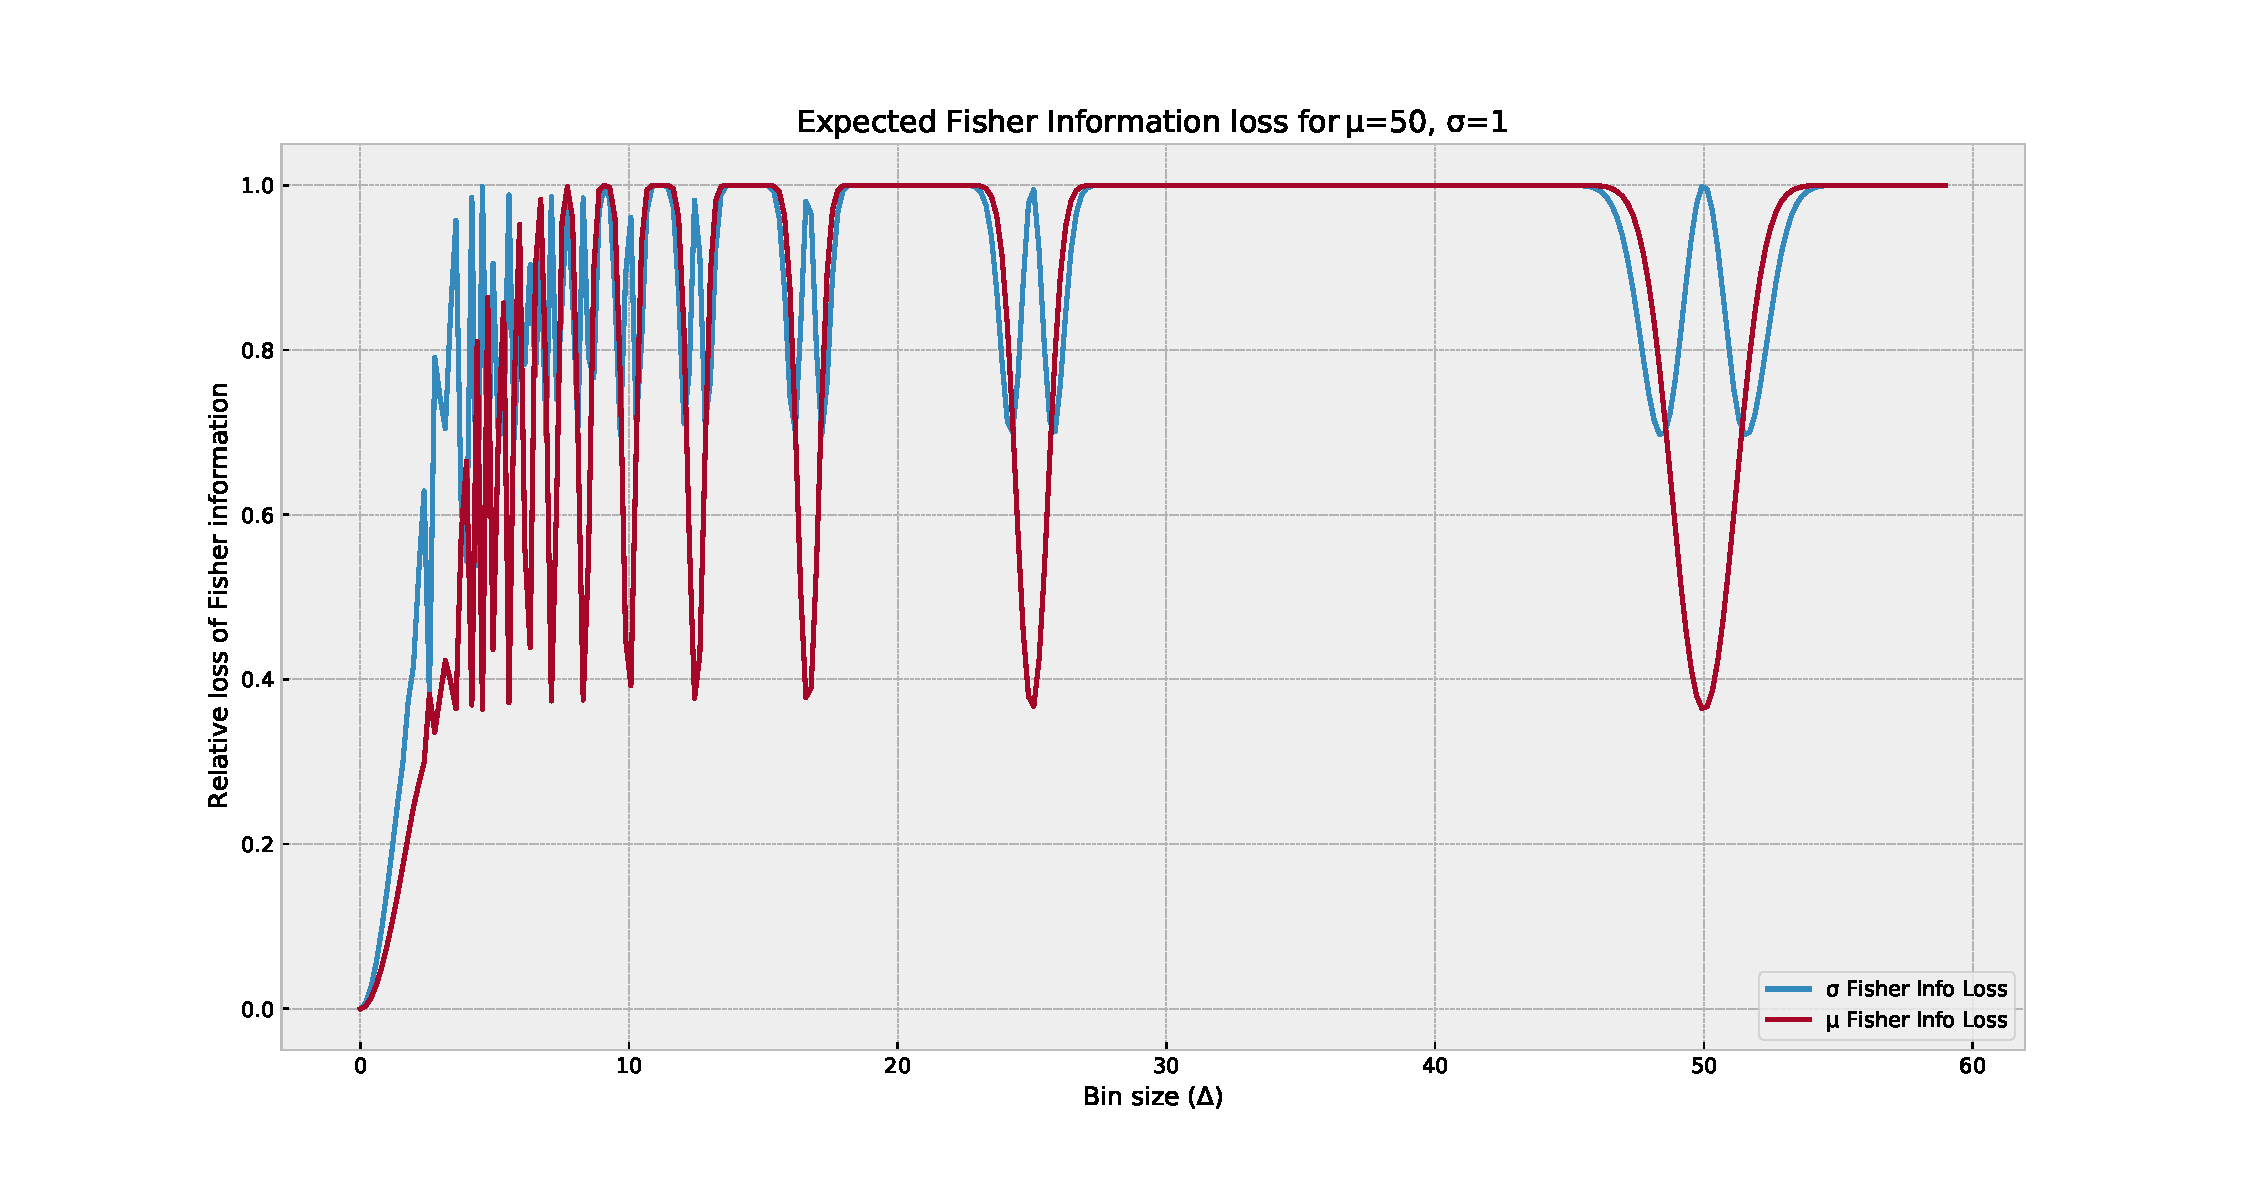
\includegraphics[height=5cm, width=6cm]{mu50sig1.pdf}
			\centering
		\end{figure}
	\end{columns}
\end{frame}

\begin{frame}
	\frametitle{Normal Aggregated MLE example}
	\begin{itemize}
		\item Run 5000 simulations of toy inference problem with $X \sim \mathcal{N}(\mu=1, \sigma=1)$ with $\sigma$ known, $\Delta=3$, and $n=500$.
		\item Variance of simulated results agree with inverse of derived Fisher Information for $\mu$. Aggregated MLE is asymptotically efficient.
	\end{itemize}
	\begin{figure}[!h]
		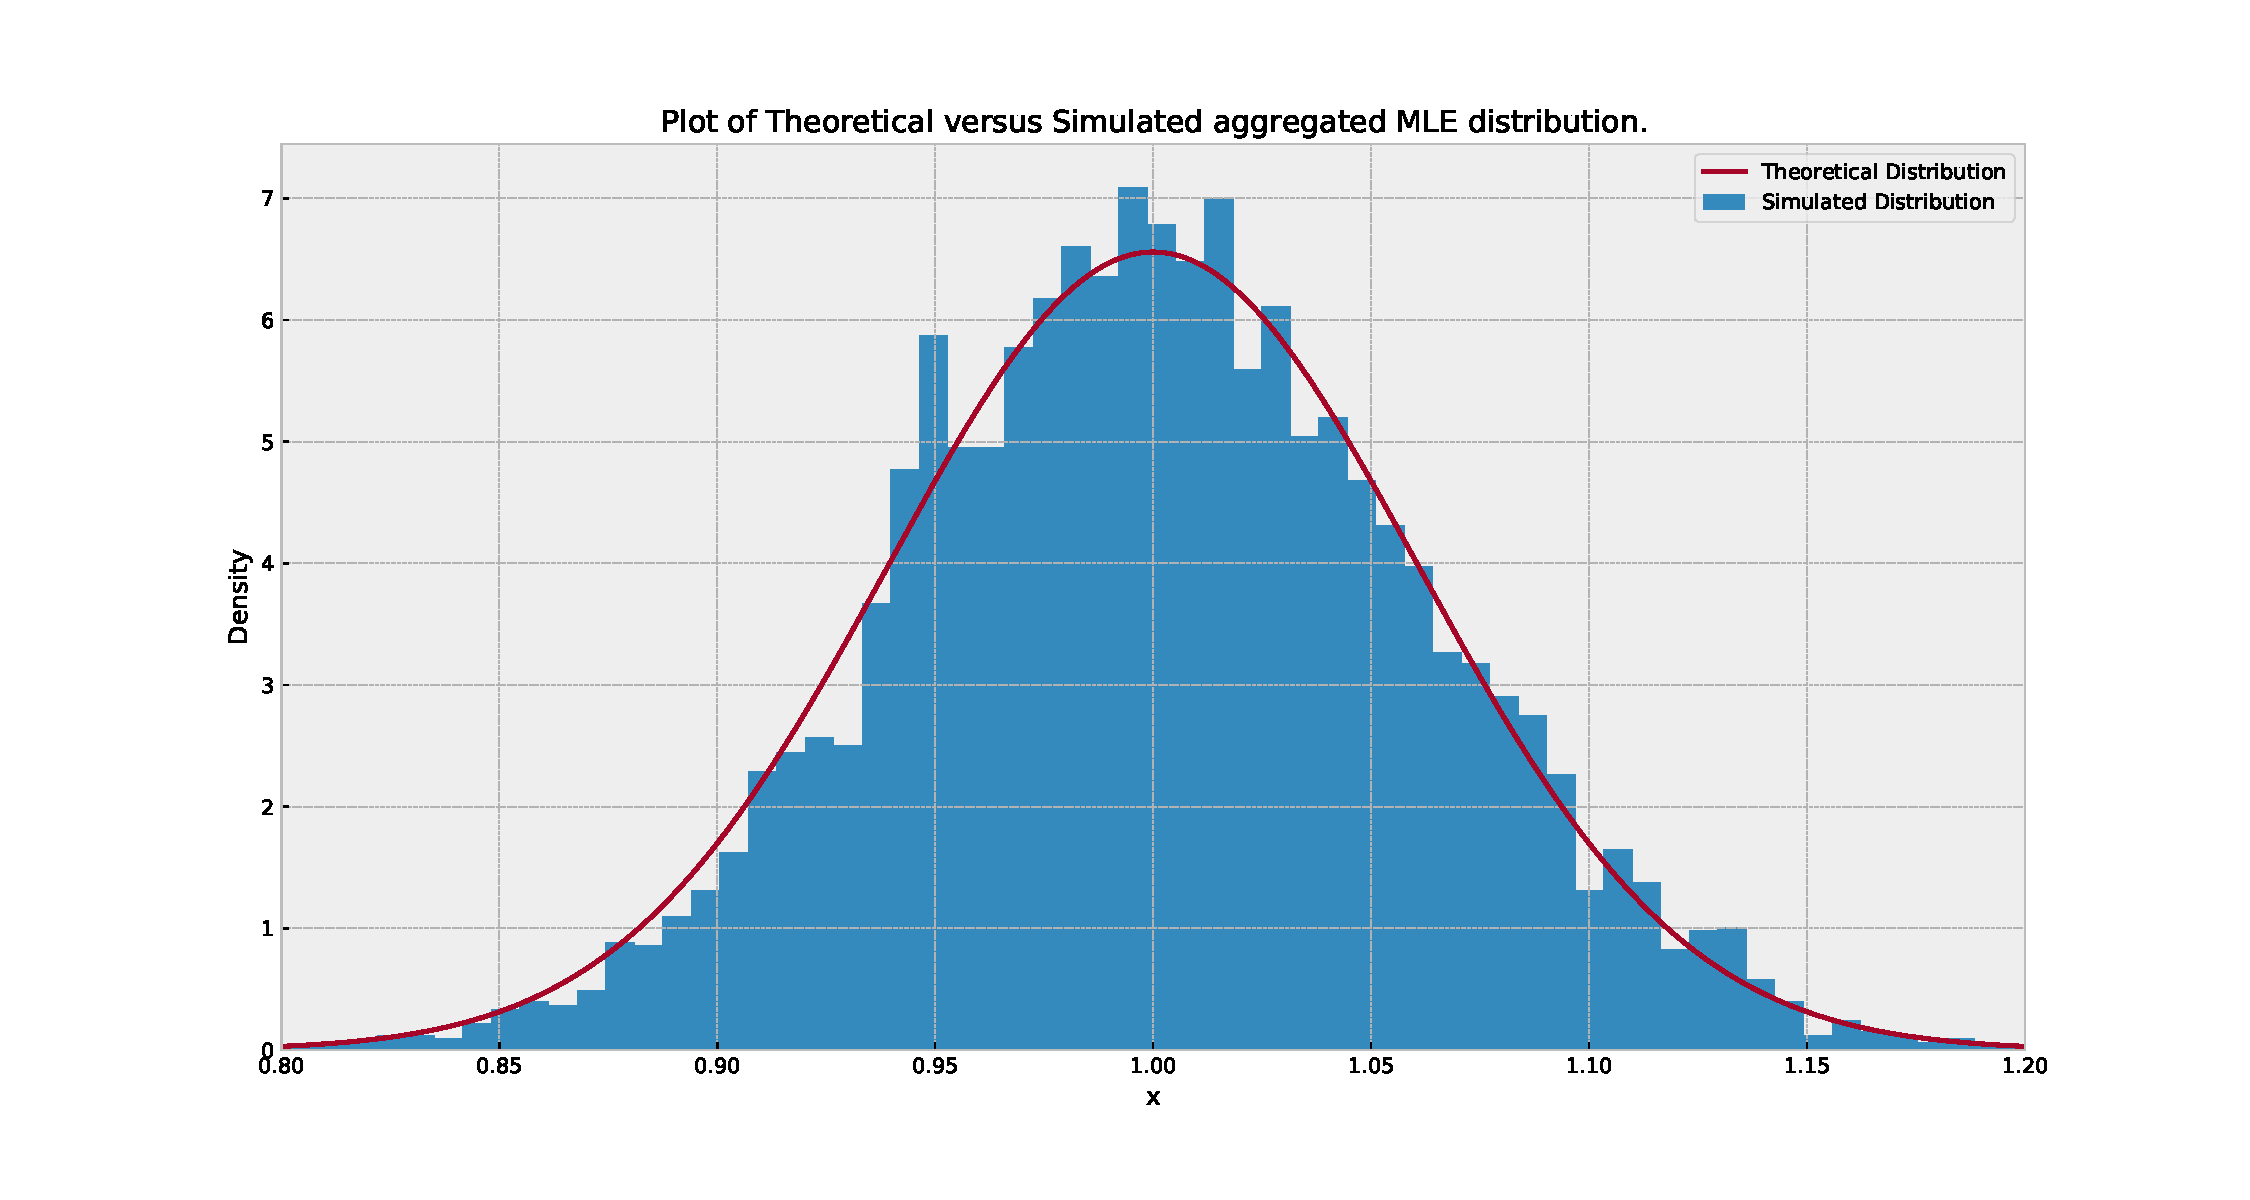
\includegraphics[height=6cm, width=12cm]{mle_distribution.pdf}
	\end{figure}
\end{frame}

\section{Inhomogeneous Poisson Processes}

\begin{frame}
	\frametitle{Poisson Process}
	\begin{itemize}
		\item Poisson processes are a simple type of counting process defined by their rate function: $\lambda(t) \geq 0$.
		\item They are homogeneous if $\lambda(t) = \lambda$ is constant; and inhomogeneous if $\lambda(t)$ is deterministic and varies through time.
		\item They have an associated intensity, or mean, function defined over any subset $A$ of the real line [\cite{daley_point_processes}]:
		\begin{equation*}
			\Lambda(A) = \int_A \lambda(t) \text{d}t.
		\end{equation*}
	\end{itemize}
\end{frame}

\begin{frame}
	\frametitle{Periodic Rate Poisson Process}
	\begin{itemize}
		\item We investigate an inhomogeneous, periodic Poisson process with rate function:
		\begin{equation*}
			\lambda(t; \omega) = 1 + \cos(\omega t).
		\end{equation*}
		\item Nyquist rate is minimum sampling rate to avoid distortion in signal processing [\cite{nyquist}]. Provides starting point for limit of resolution for periodic inference problems.
		\item For function with highest frequency $B$, Nyquist rate is $2B$. Frequency in this setting is $B = \omega / (2 \pi)$; giving Nyquist rate of $2B = \omega / \pi$.
		\item We find this provides a safe upper-limit to the level of aggregation, setting $\Delta > 2B$ can result in model unidentifiability.
	\end{itemize}
\end{frame}

\begin{frame}
	\frametitle{Periodic Rate Poisson Process - Identifiable}
	\begin{itemize}
		\item Performing inference on $\omega= \pi$, with $T=25, K=50$ and so $\Delta=0.5$.
		\item $\Delta = 0.5 < 2B = 1$, so we expect to be able to identify our model from the observations.
		\item Aggregated log-likelihood function has a clear sole maximum near the true value $\omega=\pi$, no issues with identifiability.
	\end{itemize}
	\begin{figure}[!h]
		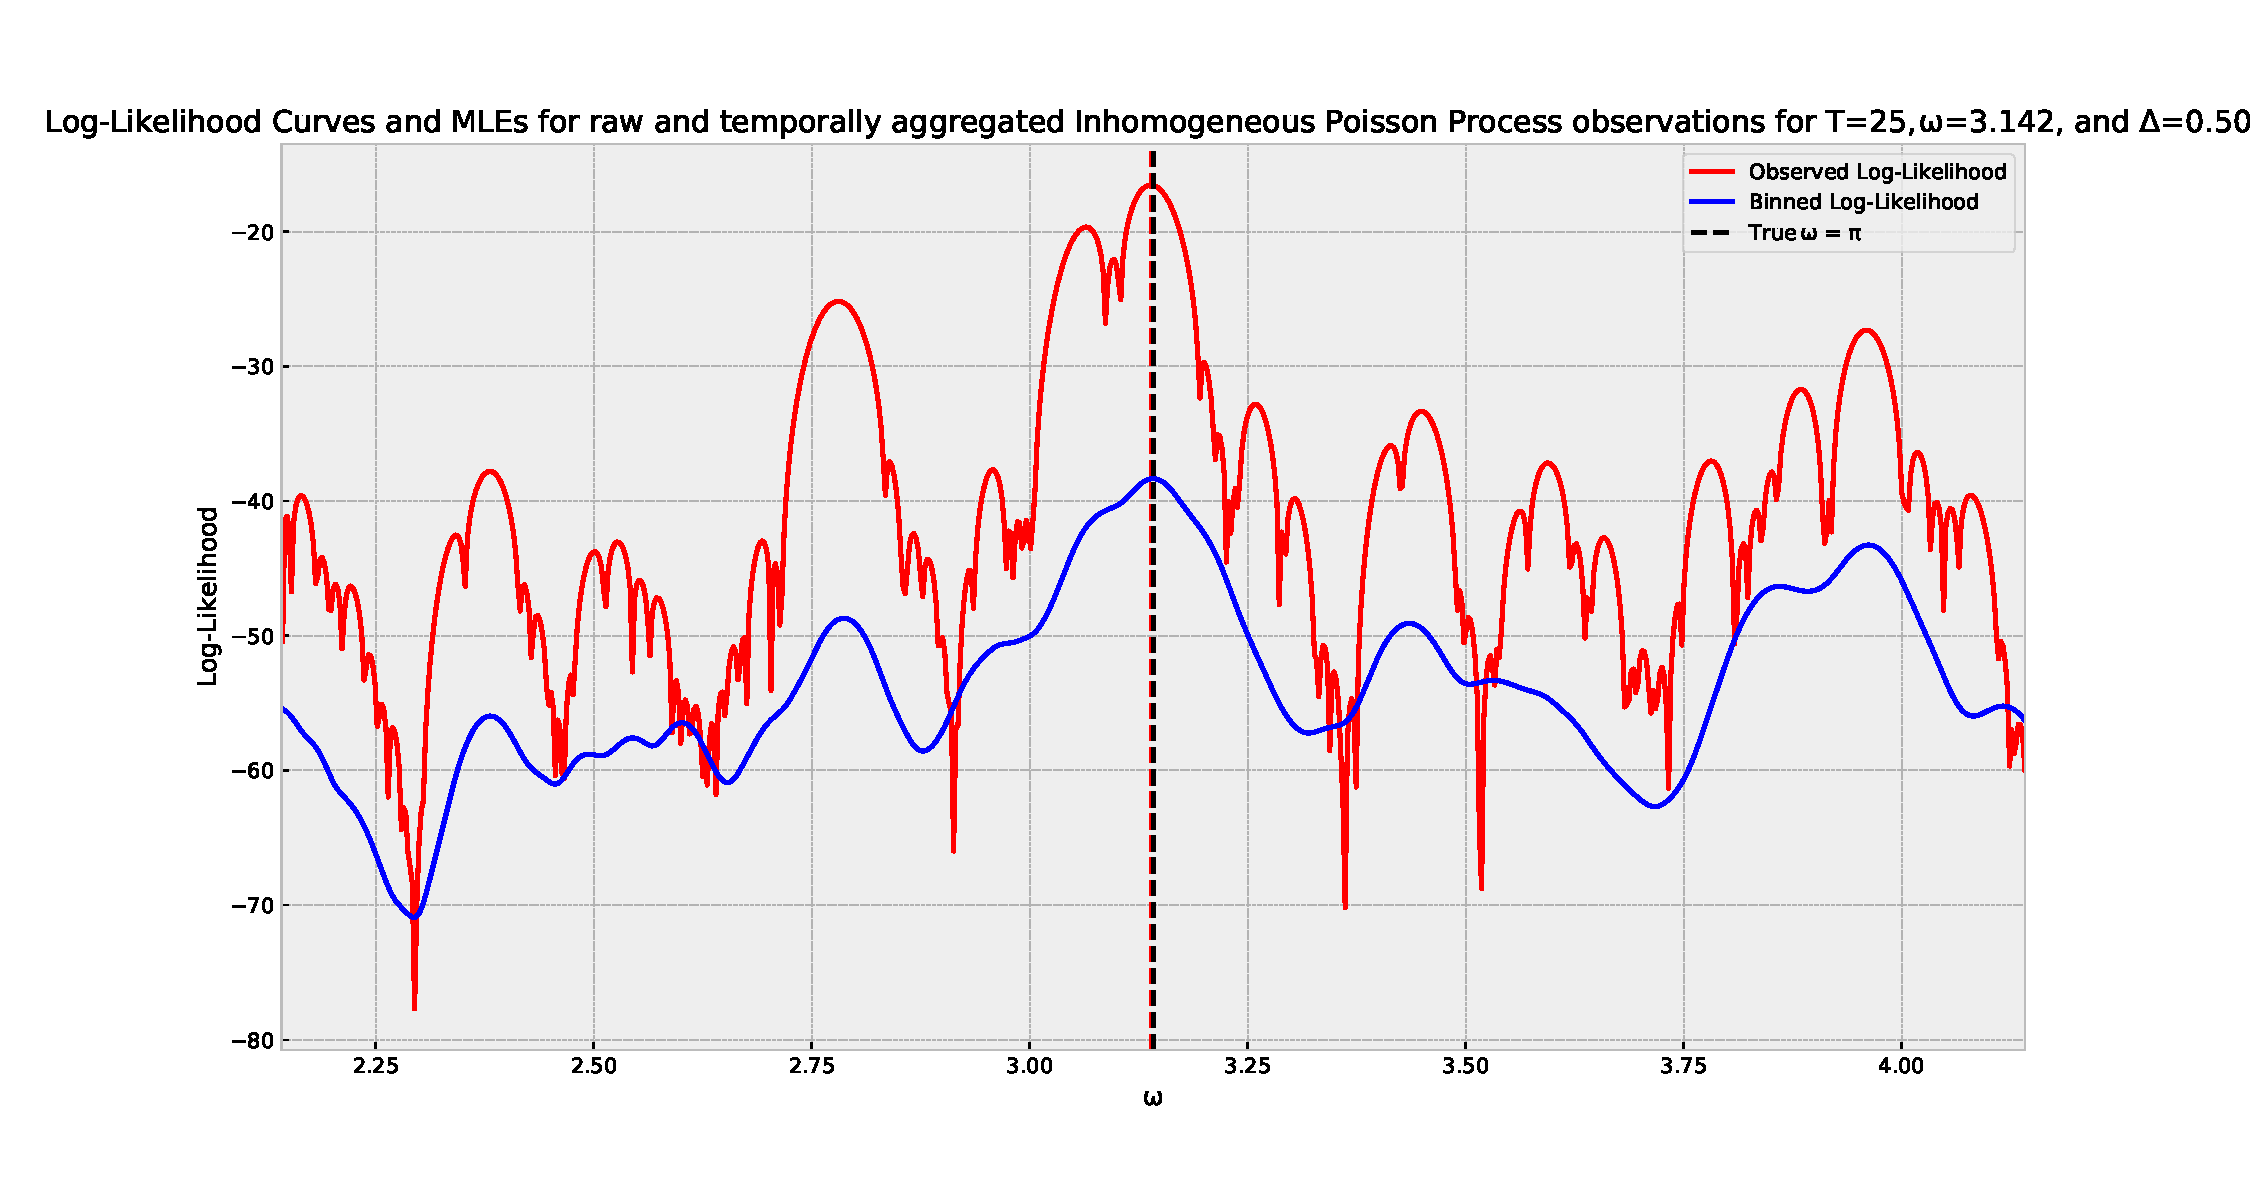
\includegraphics[height=5.5cm, width=12cm]{nhpp_periodic_id_log_likeli.pdf}
	\end{figure}
\end{frame}

\begin{frame}
	\frametitle{Periodic Rate Poisson Process - Unidentifiable}
	\begin{itemize}
		\item Again we have $\omega= \pi$, with $T=25$, now $K=13$ and so $\Delta=1.92$.
		\item $\Delta = 1.92 > 2B = 1$, expect issues with identifiability.
		\item Aggregated log-likelihood function has no clear sole maximum near the true value $\omega=\pi$. Curve is almost flat meaning we have an unidentifiable model. Inference can't be performed in this setting.
	\end{itemize}
	\begin{figure}[!h]
		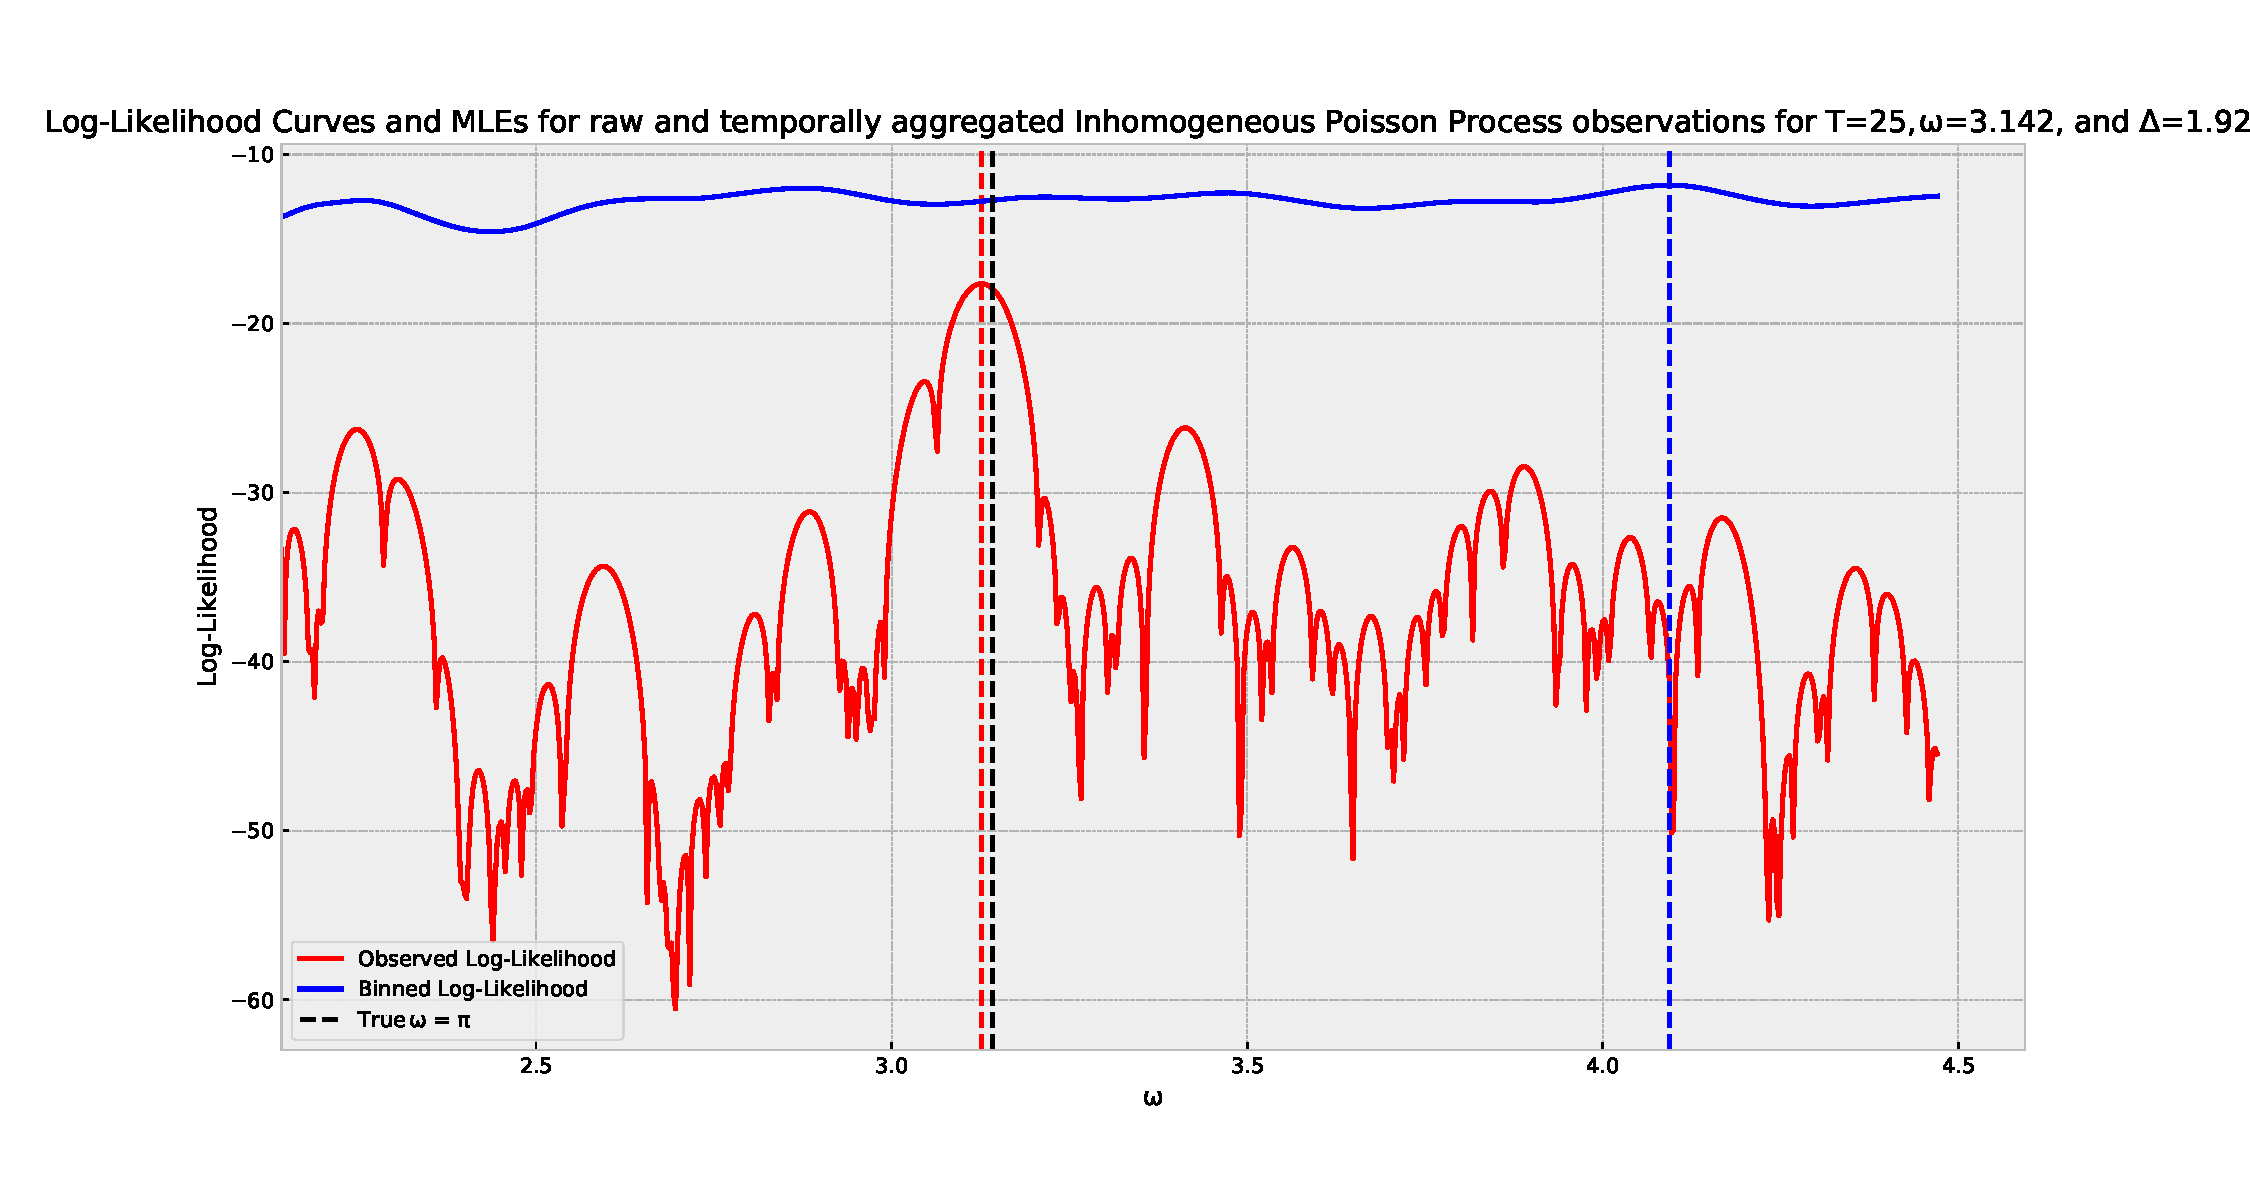
\includegraphics[height=5.5cm, width=12cm]{nhpp_periodic_unid_log_likeli.pdf}
	\end{figure}
\end{frame}

\section{Conclusion}
\begin{frame}
	\frametitle{Conclusion}
	\begin{itemize}
		\item General approach for calculating loss of Fisher Information in aggregated cases has been presented.
		\item Specific results derived for Poisson, Exponential, and Normal distributions, and for Poisson Processes.
		\item Aggregated MLE is asymptotically efficient, achieving CRLB.
		\item Issues exist with model identifiability due to over-aggregation with periodic functions.
	\end{itemize}
\end{frame}

\begin{frame}
	\frametitle{Bibliography}
	\bibliographystyle{abbrvnat} % set the bibliography style
	\bibliography{bibtexfile} % generate the bibliography
\end{frame}

\end{document}
